\setcounter{chapter}{2}
\chapter{Methods}

\section{Models}

\subsection{Introduction}
It is important to distinguish between the two model-types used in this thesis. I therefore explain both the general idea behind the model-types, and the specifics behind the models themselves. 
\subsection{\acrfull{nwp} - model}
An \acrshort{nwp}-model collects observational data for the gridded model area to get the best estimate to start a model run. When the model is ready to be run, it advances in time, calculating the state of the atmosphere for the next timestep, the state of the atmosphere is then recorded for different times (hourly for \acrshort{meps} and may then be processed. Operational \acrshort{nwp}-models are often updated when advances are ready, so models for different days can be using different physics schema. Modern \acrshort{nwp}-models also utilize pertubated ensemble-members. This is done by having a control run use the collected observational data, and then doing small (inside of the observational uncertainty range) changes or pertubations to the other runs. Each run is then a member in the whole ensemble, and the ensemble as a whole is meant to be the possible outcomes from a observed starting point.
\subsubsection{MEPS}
The operational\footnote{Note that in February 2020, both the format and frequency of model runs for \acrfull{meps} was changed considerably, operational here refers to the model-runs from 2016-2019} model used for the cases looked into in this thesis is hourly gridded $2.5x2.5$km grids with $67$-vertical model levels using the harmonie-arome (\cite{aromehirlam}). Archived data for this model-setup is available from 2016 to 2019.
\subsection{Reanalysis - model}
A reanalysis differs from an operational \acrshort{nwp}-model in that it uses a fixed version of a \acrshort{nwp}-model on historical weather observations. This is done to create the best possible historical weather data, by turning point and field observations into a complete gridded archive of historical weather. Reanalysis models may also be run with pertubated ensembles, to capture variation between the times when observational data is concidered.
\subsubsection{ERA5}
The \acrfull{era5} dataset is created by the \acrfull{ecmwf} and provides hourly data, in $31x31$km grids, with $137$ vertical model-levels. The data ranges from $1979$ to and including $2019$ (It is continually updated as I write this, so it is probably updated beyond 2019). The observational data is assimilated in 12-hour windows \cite{era5}
I will be utilizing the \acrshort{era5} dataset to create a set of climatologies and case-based atmospheric conditions, using the data reported on pressure levels (see Appendix A about model level/pressure level discussion). 
\subsection{How is HTL forecast today?}
%In 1999 there was a research project awarded to AEA Technology \cite{hardwick} and the British Met. Office, where they investigated the probable causes and spatial spread of \acrshort{htl}. There is also an important study done by Wilkinson (\cite{wilkinson}), which adds numerical weather prediction aspects to this.  In my thesis, I apply more state-of-the-art numerical weather prediction models to build on these earlier studies. 
The operational forecast as of today, is based on findings by \cite{hardwick} and \cite{wilkinson}. It assigns a risk or \acrfull{hti}  in percentage based on four meteorological factors:
\begin{itemize}
    \item Vertical wind speed in the altitude that helicopters generally fly in
    \item Temperature at the altitude that helicopters generally fly in
    \item Total precipitation during the last hour
    \item Amount of low clouds in the surrounding area
\end{itemize}
This risk is an index designed to forecast local and shallow convective activity, and I will in this thesis also look at how well this risk captures the actual danger.
The index is categorized in four different classes of severity, from no danger (White) to very high risk (Red). (See figure \ref{fig:hti}).
\begin{itemize}
    \item White: $HTI < 0.73$
    \item Yellow: $0.73 \leq HTI < 0.90 $
    \item Brown: $0.90 \leq HTI < 0.99 $
    \item Red: $0.99 \leq HTI $
\end{itemize}
The severity-categories are based on discussion with the helicopter operators in Norway (Bristow and CHC), and is changed after yearly evaluation. \acrshort{hti} is not based on a regression analysis, but rather a subjective review of the earlier cases of incidents.
\begin{figure}
    \centering
    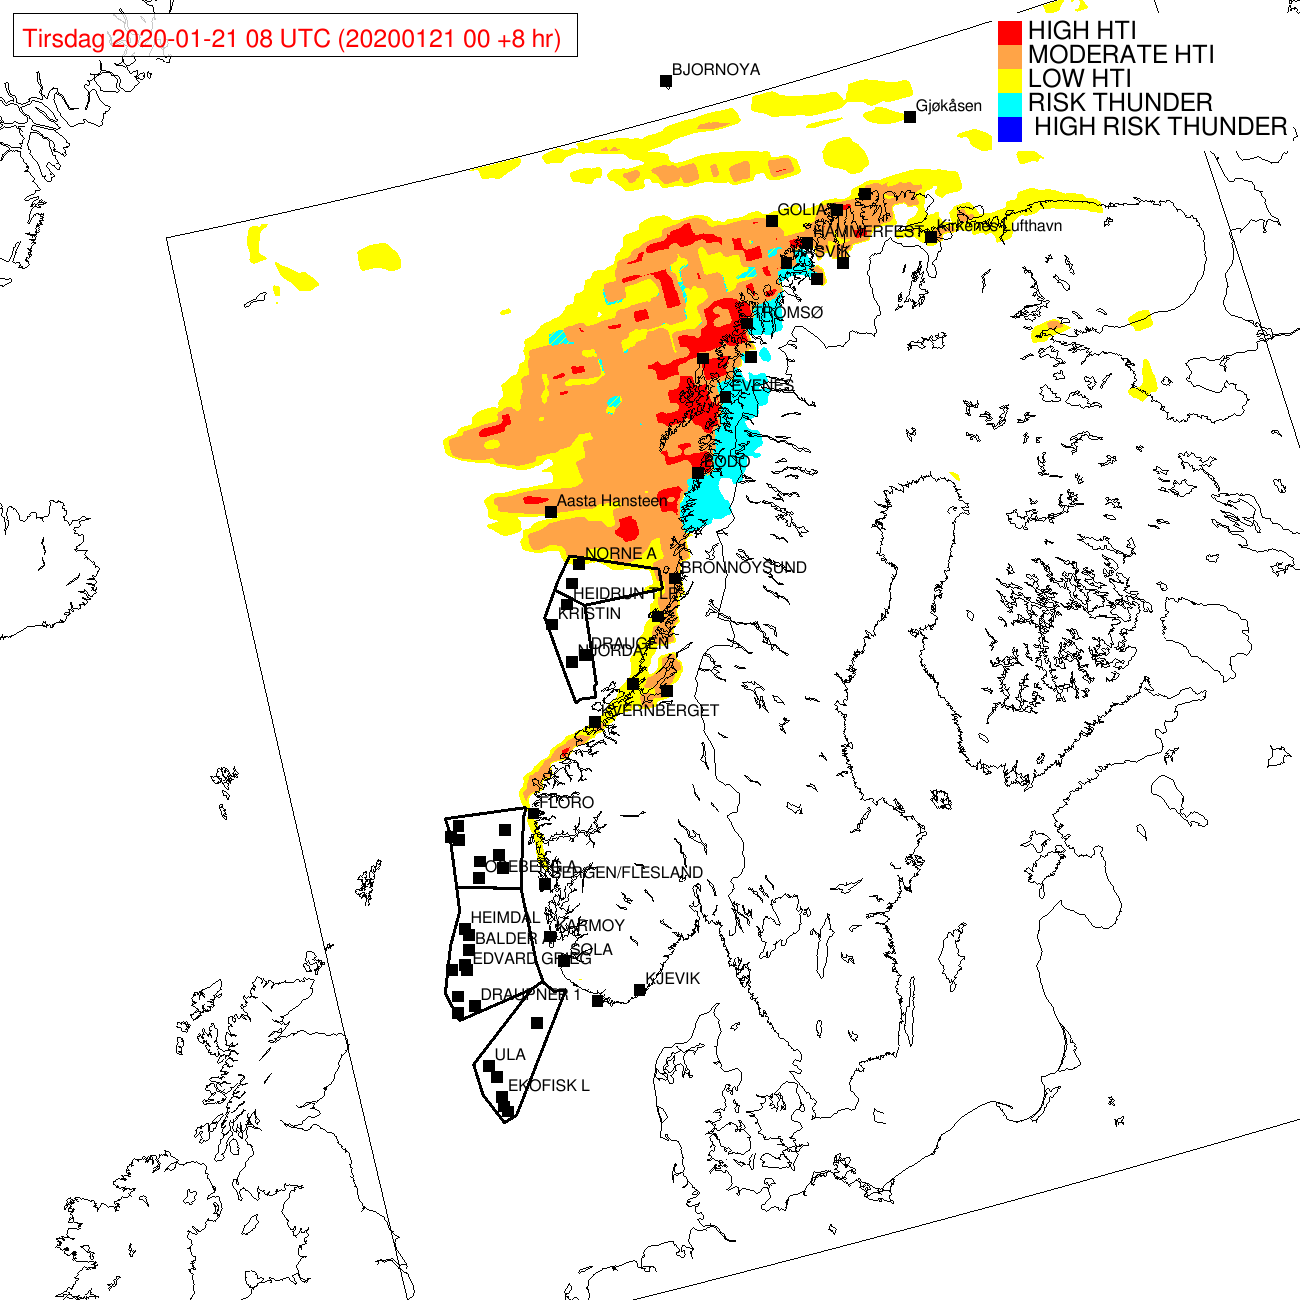
\includegraphics[width=\textwidth]{Figures/hti.png}
    \caption{Screenshot from https://www.ippc.no for 21. of January 2020, showing the HTI-forecast with 8 hour lead-time after midnight. The blue thunder-cells show another forecast-product from MET, forecasting risk for natural lightning. A plane was hit by lightning, and was therefore diverted from flying into Bodø during this forecasts valid time. }
    \label{fig:hti}
\end{figure}
\section{Data}

\subsection{Incidents from Avinor}
I have received a dataset from Avinor, which I have gridded based on the pilots’ reports on position during incidents. This data included all reports on incidents received by AVINOR pertaining to lightning. I have filtered out cases where there was observed lightning in the area and not striking the aircraft, to prevent warm-season lightning to muddle the data. This dataset includes both fixed-wing and helicopters. 

\begin{table}
\begin{tabular}{ l|c|c|c|c| } 
		&Total cases & Height info & Position & Reported temperature (OAT) \\
 		\hline
 		Helicopters &$40$ & $37$ & $24$ & $12$\\ 
 		Fixed-wing &$256$ & $217$ & $256$ & $1$\\ 
 		\hline
 		Total &$296$ &$254$ & $280$ & $13$\\ 
 		\hline
\end{tabular}
\caption{Data available for each case in the Avinor-dataset. Note that there is one helicopter case where height is not known, but position is. }
\label{tab:avinor}
\end{table}

\subsection{Weather report from airports - METAR}


\subsection{Lightning - UALF}

\section{Tools}
To investigate and quantify the different parts of the operational forecast, I have created a Python class that relies on the Python-module xarray to perform different post-prossesing algorithms. During my preliminary testing of this tool, I discovered a bug in the operational \acrshort{htl}-forecast. I therefore also look into the effects of this bug for the forecast as a whole and in special cases (Possible over-assessing risk on northern-facing coastal areas). Further, this tool gives me the possibility to produce forecasts for larger ensembles, making it  possible improvements done by using the whole ensemble and not just the control run.
